% Options for packages loaded elsewhere
\PassOptionsToPackage{unicode}{hyperref}
\PassOptionsToPackage{hyphens}{url}
%
\documentclass[
  11pt,
  ignorenonframetext,
]{beamer}
\usepackage{pgfpages}
\setbeamertemplate{caption}[numbered]
\setbeamertemplate{caption label separator}{: }
\setbeamercolor{caption name}{fg=normal text.fg}
\beamertemplatenavigationsymbolsempty
% Prevent slide breaks in the middle of a paragraph
\widowpenalties 1 10000
\raggedbottom
\setbeamertemplate{part page}{
  \centering
  \begin{beamercolorbox}[sep=16pt,center]{part title}
    \usebeamerfont{part title}\insertpart\par
  \end{beamercolorbox}
}
\setbeamertemplate{section page}{
  \centering
  \begin{beamercolorbox}[sep=12pt,center]{part title}
    \usebeamerfont{section title}\insertsection\par
  \end{beamercolorbox}
}
\setbeamertemplate{subsection page}{
  \centering
  \begin{beamercolorbox}[sep=8pt,center]{part title}
    \usebeamerfont{subsection title}\insertsubsection\par
  \end{beamercolorbox}
}
\AtBeginPart{
  \frame{\partpage}
}
\AtBeginSection{
  \ifbibliography
  \else
    \frame{\sectionpage}
  \fi
}
\AtBeginSubsection{
  \frame{\subsectionpage}
}
\usepackage{amsmath,amssymb}
\usepackage{lmodern}
\usepackage{iftex}
\ifPDFTeX
  \usepackage[T1]{fontenc}
  \usepackage[utf8]{inputenc}
  \usepackage{textcomp} % provide euro and other symbols
\else % if luatex or xetex
  \usepackage{unicode-math}
  \defaultfontfeatures{Scale=MatchLowercase}
  \defaultfontfeatures[\rmfamily]{Ligatures=TeX,Scale=1}
\fi
\usetheme[]{metropolis}
% Use upquote if available, for straight quotes in verbatim environments
\IfFileExists{upquote.sty}{\usepackage{upquote}}{}
\IfFileExists{microtype.sty}{% use microtype if available
  \usepackage[]{microtype}
  \UseMicrotypeSet[protrusion]{basicmath} % disable protrusion for tt fonts
}{}
\makeatletter
\@ifundefined{KOMAClassName}{% if non-KOMA class
  \IfFileExists{parskip.sty}{%
    \usepackage{parskip}
  }{% else
    \setlength{\parindent}{0pt}
    \setlength{\parskip}{6pt plus 2pt minus 1pt}}
}{% if KOMA class
  \KOMAoptions{parskip=half}}
\makeatother
\usepackage{xcolor}
\newif\ifbibliography
\usepackage{color}
\usepackage{fancyvrb}
\newcommand{\VerbBar}{|}
\newcommand{\VERB}{\Verb[commandchars=\\\{\}]}
\DefineVerbatimEnvironment{Highlighting}{Verbatim}{commandchars=\\\{\}}
% Add ',fontsize=\small' for more characters per line
\newenvironment{Shaded}{}{}
\newcommand{\AlertTok}[1]{\textcolor[rgb]{1.00,0.00,0.00}{\textbf{#1}}}
\newcommand{\AnnotationTok}[1]{\textcolor[rgb]{0.38,0.63,0.69}{\textbf{\textit{#1}}}}
\newcommand{\AttributeTok}[1]{\textcolor[rgb]{0.49,0.56,0.16}{#1}}
\newcommand{\BaseNTok}[1]{\textcolor[rgb]{0.25,0.63,0.44}{#1}}
\newcommand{\BuiltInTok}[1]{\textcolor[rgb]{0.00,0.50,0.00}{#1}}
\newcommand{\CharTok}[1]{\textcolor[rgb]{0.25,0.44,0.63}{#1}}
\newcommand{\CommentTok}[1]{\textcolor[rgb]{0.38,0.63,0.69}{\textit{#1}}}
\newcommand{\CommentVarTok}[1]{\textcolor[rgb]{0.38,0.63,0.69}{\textbf{\textit{#1}}}}
\newcommand{\ConstantTok}[1]{\textcolor[rgb]{0.53,0.00,0.00}{#1}}
\newcommand{\ControlFlowTok}[1]{\textcolor[rgb]{0.00,0.44,0.13}{\textbf{#1}}}
\newcommand{\DataTypeTok}[1]{\textcolor[rgb]{0.56,0.13,0.00}{#1}}
\newcommand{\DecValTok}[1]{\textcolor[rgb]{0.25,0.63,0.44}{#1}}
\newcommand{\DocumentationTok}[1]{\textcolor[rgb]{0.73,0.13,0.13}{\textit{#1}}}
\newcommand{\ErrorTok}[1]{\textcolor[rgb]{1.00,0.00,0.00}{\textbf{#1}}}
\newcommand{\ExtensionTok}[1]{#1}
\newcommand{\FloatTok}[1]{\textcolor[rgb]{0.25,0.63,0.44}{#1}}
\newcommand{\FunctionTok}[1]{\textcolor[rgb]{0.02,0.16,0.49}{#1}}
\newcommand{\ImportTok}[1]{\textcolor[rgb]{0.00,0.50,0.00}{\textbf{#1}}}
\newcommand{\InformationTok}[1]{\textcolor[rgb]{0.38,0.63,0.69}{\textbf{\textit{#1}}}}
\newcommand{\KeywordTok}[1]{\textcolor[rgb]{0.00,0.44,0.13}{\textbf{#1}}}
\newcommand{\NormalTok}[1]{#1}
\newcommand{\OperatorTok}[1]{\textcolor[rgb]{0.40,0.40,0.40}{#1}}
\newcommand{\OtherTok}[1]{\textcolor[rgb]{0.00,0.44,0.13}{#1}}
\newcommand{\PreprocessorTok}[1]{\textcolor[rgb]{0.74,0.48,0.00}{#1}}
\newcommand{\RegionMarkerTok}[1]{#1}
\newcommand{\SpecialCharTok}[1]{\textcolor[rgb]{0.25,0.44,0.63}{#1}}
\newcommand{\SpecialStringTok}[1]{\textcolor[rgb]{0.73,0.40,0.53}{#1}}
\newcommand{\StringTok}[1]{\textcolor[rgb]{0.25,0.44,0.63}{#1}}
\newcommand{\VariableTok}[1]{\textcolor[rgb]{0.10,0.09,0.49}{#1}}
\newcommand{\VerbatimStringTok}[1]{\textcolor[rgb]{0.25,0.44,0.63}{#1}}
\newcommand{\WarningTok}[1]{\textcolor[rgb]{0.38,0.63,0.69}{\textbf{\textit{#1}}}}
\usepackage{graphicx}
\makeatletter
\def\maxwidth{\ifdim\Gin@nat@width>\linewidth\linewidth\else\Gin@nat@width\fi}
\def\maxheight{\ifdim\Gin@nat@height>\textheight\textheight\else\Gin@nat@height\fi}
\makeatother
% Scale images if necessary, so that they will not overflow the page
% margins by default, and it is still possible to overwrite the defaults
% using explicit options in \includegraphics[width, height, ...]{}
\setkeys{Gin}{width=\maxwidth,height=\maxheight,keepaspectratio}
% Set default figure placement to htbp
\makeatletter
\def\fps@figure{htbp}
\makeatother
\setlength{\emergencystretch}{3em} % prevent overfull lines
\providecommand{\tightlist}{%
  \setlength{\itemsep}{0pt}\setlength{\parskip}{0pt}}
\setcounter{secnumdepth}{-\maxdimen} % remove section numbering
\ifLuaTeX
  \usepackage{selnolig}  % disable illegal ligatures
\fi
\IfFileExists{bookmark.sty}{\usepackage{bookmark}}{\usepackage{hyperref}}
\IfFileExists{xurl.sty}{\usepackage{xurl}}{} % add URL line breaks if available
\urlstyle{same} % disable monospaced font for URLs
\hypersetup{
  pdftitle={Análisis de la asociación espacial},
  pdfauthor={Gerardo Martín},
  hidelinks,
  pdfcreator={LaTeX via pandoc}}

\title{Análisis de la asociación espacial}
\subtitle{Asociación con el espacio}
\author{Gerardo Martín}
\date{2022-06-29}

\begin{document}
\frame{\titlepage}

\begin{frame}{Intro}
\protect\hypertarget{intro}{}
Anteriormente:

\begin{itemize}
\tightlist
\item
  Asociación entre dos procesos espaciales
\end{itemize}

Ahora

\begin{itemize}
\item
  Asociación de un proceso con el espacio:

  \begin{itemize}
  \tightlist
  \item
    Ubicación en el plano cartesiano
  \item
    En relación a unidades espaciales vecinas
  \end{itemize}
\end{itemize}
\end{frame}

\begin{frame}{Ejemplos}
\protect\hypertarget{ejemplos}{}
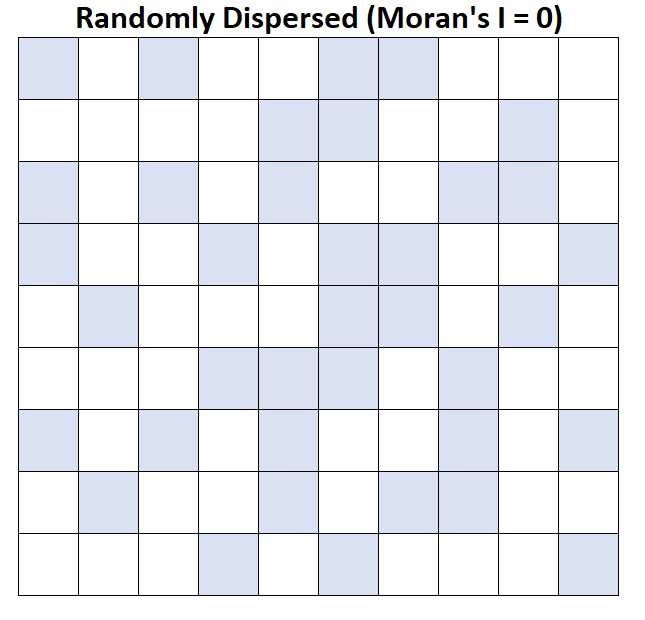
\includegraphics{Asociacion-imagenes/morani1.png}
\end{frame}

\begin{frame}{Ejemplos}
\protect\hypertarget{ejemplos-1}{}
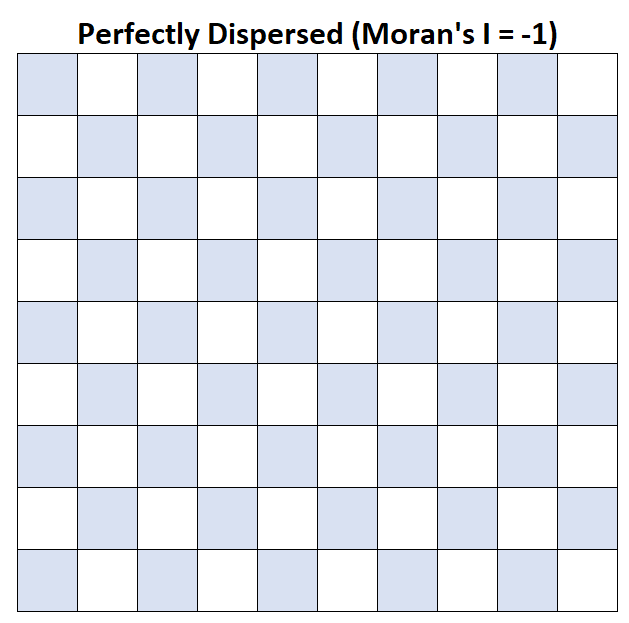
\includegraphics{Asociacion-imagenes/morani2.png}
\end{frame}

\begin{frame}{Ejemplo}
\protect\hypertarget{ejemplo}{}
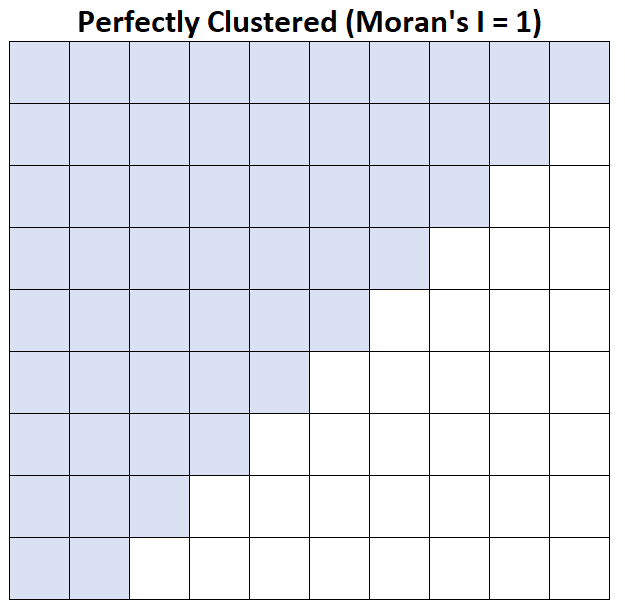
\includegraphics{Asociacion-imagenes/morani3.png}
\end{frame}

\begin{frame}{Índice \textbf{I} de Moran}
\protect\hypertarget{uxedndice-i-de-moran}{}
Medición de la agregación de valores similares

\begin{equation}
    I = N \times W \times \sum_{i = 1}^n \sum_{j = 1}^n w_{ij} \frac{(x_i - \bar{x})(x_j - \bar{x})}{\sum (x_i - \bar{x})^2}
\end{equation}
\end{frame}

\begin{frame}{Índice \emph{I} de Moran}
\protect\hypertarget{uxedndice-i-de-moran-1}{}
\begin{itemize}
\tightlist
\item
  \(N\) es el número total de unidades espaciales indizadas por \(i\) y
  \(j\)
\item
  \(W\) es la suma de pesos \(w_{ij}\)
\item
  \(x\) es la variable de interés
\item
  \(\bar{x}\) es la media de \(x\)
\item
  \(w_{ij}\) es una matriz de pesos espaciales
\end{itemize}
\end{frame}

\begin{frame}{Indización de las unidades}
\protect\hypertarget{indizaciuxf3n-de-las-unidades}{}
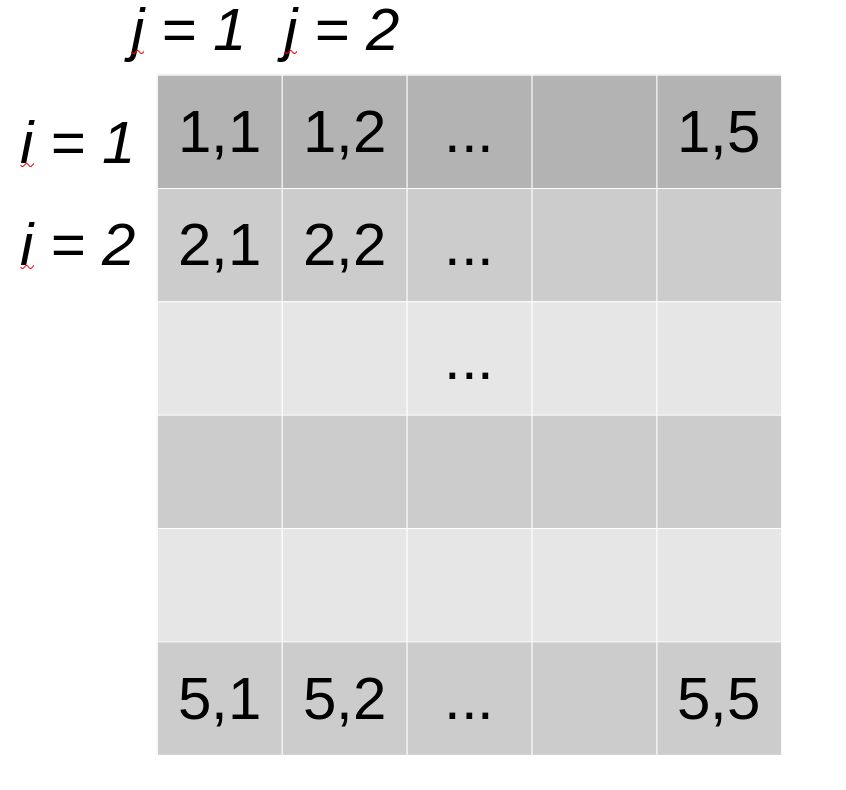
\includegraphics{Asociacion-imagenes/indizacion.png}
\end{frame}

\begin{frame}{Interpretación de \emph{I} de Moran}
\protect\hypertarget{interpretaciuxf3n-de-i-de-moran}{}
\(I = 0\), valores son aleatorios, no hay asociación con espacio

\(I = 1\), Valores están perfectamente dispersos

\(I=-1\), Valores están perfectamente agregados
\end{frame}

\hypertarget{implementaciuxf3n-en-r}{%
\section{\texorpdfstring{Implementación en
\textbf{R}}{Implementación en R}}\label{implementaciuxf3n-en-r}}

\begin{frame}[fragile]{Para datos raster}
\protect\hypertarget{para-datos-raster}{}
Función \texttt{Moran}, argumento: objeto que contiene capa raster

\begin{Shaded}
\begin{Highlighting}[]
\FunctionTok{library}\NormalTok{(raster)}
\NormalTok{r }\OtherTok{\textless{}{-}} \FunctionTok{raster}\NormalTok{(}\StringTok{"../Datos{-}ejemplos/Var{-}1.tif"}\NormalTok{)}
\FunctionTok{Moran}\NormalTok{(r)}
\end{Highlighting}
\end{Shaded}

\begin{verbatim}
## [1] 0.78433
\end{verbatim}
\end{frame}

\begin{frame}{La capa analizada}
\protect\hypertarget{la-capa-analizada}{}
\begin{center}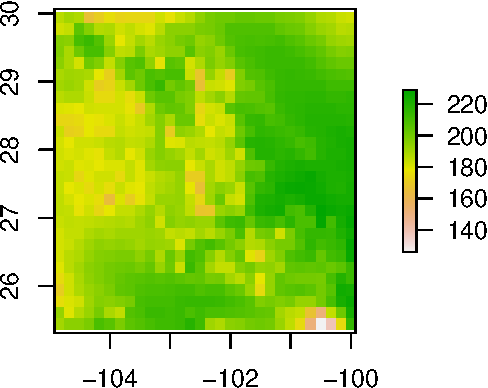
\includegraphics{Asociacion-espacio_files/figure-beamer/unnamed-chunk-2-1} \end{center}
\end{frame}

\begin{frame}[fragile]{Otro ejemplo}
\protect\hypertarget{otro-ejemplo}{}
Reemplazaremos valores de \texttt{r} con otros de distribución uniforme:

\begin{Shaded}
\begin{Highlighting}[]
\FunctionTok{set.seed}\NormalTok{(}\DecValTok{5934857}\NormalTok{)}
\NormalTok{r1 }\OtherTok{\textless{}{-}}\NormalTok{ r}
\NormalTok{r1[] }\OtherTok{\textless{}{-}} \FunctionTok{runif}\NormalTok{(}\FunctionTok{ncell}\NormalTok{(r))}
\FunctionTok{Moran}\NormalTok{(r1)}
\end{Highlighting}
\end{Shaded}

\begin{verbatim}
## [1] -0.01034548
\end{verbatim}
\end{frame}

\begin{frame}{La capa}
\protect\hypertarget{la-capa}{}
\begin{center}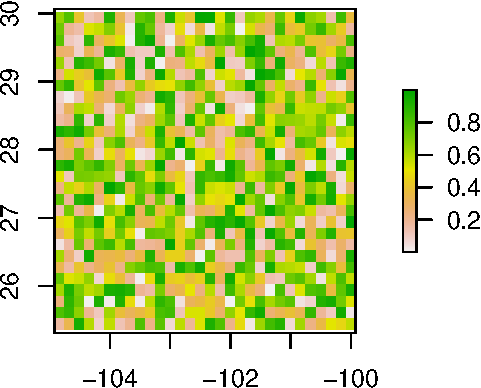
\includegraphics{Asociacion-espacio_files/figure-beamer/unnamed-chunk-4-1} \end{center}
\end{frame}

\begin{frame}{Para puntos}
\protect\hypertarget{para-puntos}{}
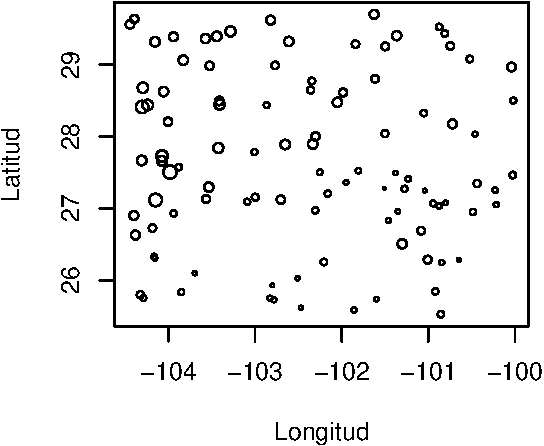
\includegraphics{Asociacion-espacio_files/figure-beamer/unnamed-chunk-5-1.pdf}
\end{frame}

\begin{frame}{Vecindades}
\protect\hypertarget{vecindades}{}
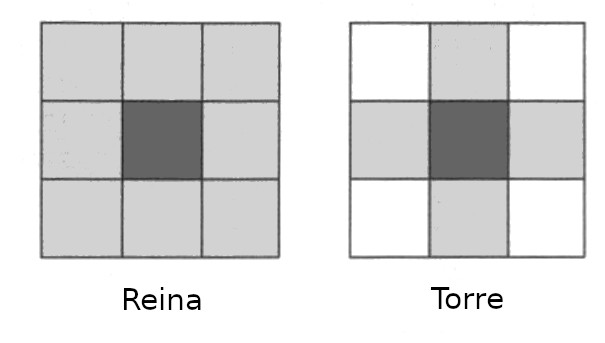
\includegraphics{Asociacion-imagenes/Reina-Torre.jpg}
\end{frame}

\begin{frame}[fragile]{Estableciendo vecindades para puntos}
\protect\hypertarget{estableciendo-vecindades-para-puntos}{}
\begin{enumerate}
\tightlist
\item
  Instalación y carga de paquete:
\end{enumerate}

\begin{Shaded}
\begin{Highlighting}[]
\FunctionTok{library}\NormalTok{(spdep)}
\end{Highlighting}
\end{Shaded}

\begin{Shaded}
\begin{Highlighting}[]
\NormalTok{vecindad }\OtherTok{\textless{}{-}} \FunctionTok{dnearneigh}\NormalTok{(}\AttributeTok{x =} \FunctionTok{as.matrix}\NormalTok{(datos[, }\FunctionTok{c}\NormalTok{(}\StringTok{"Longitud"}\NormalTok{, }\StringTok{"Latitud"}\NormalTok{)]), }\AttributeTok{d1 =} \DecValTok{0}\NormalTok{, }\AttributeTok{d2 =} \DecValTok{75}\NormalTok{, }\AttributeTok{longlat =}\NormalTok{ T)}
\NormalTok{vec.listw }\OtherTok{\textless{}{-}} \FunctionTok{nb2listw}\NormalTok{(vecindad)}
\CommentTok{\#S0 \textless{}{-} sum(nb2mat(vecindad))}
\end{Highlighting}
\end{Shaded}

\begin{itemize}
\tightlist
\item
  \texttt{x} son las coordenadas
\item
  \texttt{d1,\ d2}, distancias mínimas y máximas para considerar que
  puntos son vecinos
\item
  \texttt{longlat}, si coordenadas son en grados
\end{itemize}
\end{frame}

\begin{frame}[fragile]{Cálculo de I}
\protect\hypertarget{cuxe1lculo-de-i}{}
Necesitamos una implementación diferente, \texttt{moran.test}:

\begin{Shaded}
\begin{Highlighting}[]
\NormalTok{I.puntos }\OtherTok{\textless{}{-}} \FunctionTok{moran.test}\NormalTok{(}\AttributeTok{x =}\NormalTok{ datos}\SpecialCharTok{$}\NormalTok{Mediciones, }\AttributeTok{listw =}\NormalTok{ vec.listw)}
\end{Highlighting}
\end{Shaded}

\begin{itemize}
\item
  \texttt{x}, valores cuya correlación queremos medir
\item
  \texttt{listw}, lista de vecindades
\end{itemize}
\end{frame}

\begin{frame}[fragile]{Resultado}
\protect\hypertarget{resultado}{}
\begin{verbatim}
## 
##  Moran I test under randomisation
## 
## data:  datos$Mediciones  
## weights: vec.listw    
## 
## Moran I statistic standard deviate = 9.7604, p-value < 2.2e-16
## alternative hypothesis: greater
## sample estimates:
## Moran I statistic       Expectation          Variance 
##       0.556186118      -0.010101010       0.003366211
\end{verbatim}
\end{frame}

\end{document}
